\section{Task 3 Performance Modelling and Calibration} 

\subsection{Outline}
We will give a performance model under certain assumpton in subsection "Performance Model".
Then we will design some experiments and compare the performance model with experiments.

The final results are $t_s = 18.3\mu$s, $t_w = 56.5$ns and $t_f = 8.69$ns.

\subsection{Performance Model}
We neglect the startup overhead, including reading command line parameters, setting simulation parameters and setting initial condition.
In this case, this overall cost of this program can be divided into two terms, namely communication cost and computation cost.
All the communications happen in \lstinline{updateBoundary(w,*u,ldu)}, since there is no additional final collective communications to gather all
the flow field to the "root" process. All the computation happens in \lstinline{updateAdvectField(m,n,*u,ldu)}, since we have neglect the startup
overhead.

We assume that $P=1$, and leave the case $P \neq 1$ to next section. We also assume $Q$ is larger than $1$. If not,
it will not be a parallel program any more, which is not our interest. Therefore, there are only two communications
(left-right communication) per iteration. Since periodic boundary condition (wrap) is applied to the top-bottom direction,
so some additional assignment operations will be introduced in each iteration. However, the cost of these operations is 
negligible comparing to the cost in Lax-Wendroff algorithm, so we will not consider them in the following analysis.
We also only consider the Store and Forward (SF) routing mechanism.

The communication cost and computation cost read
\begin{eqnarray*}
	t_{\textrm{comp}} &=& M_{\textrm{loc}} \cdot N_{\textrm{loc}} \cdot t_f \\
	t_{\textrm{comm}} &=& 2 \left[ t_s + M_{\textrm{loc}} \cdot t_w  \right] 
\end{eqnarray*}
where $t_f$ is the time per element computation time for the serial advection solver, which contains $23$ FLOPS and several integer operations.
$t_w$ is the communication cost per \textit{double precision number} (not word! if use word, there should be a multipler).
$t_s$ is the communication startup time.
$t_{\textrm{comp}}$ and $t_{\textrm{comm}}$ are communication time and computation time for one simulation time step, respectively.
$N_{loc} = N/Q$ and $M_{loc}= M/P = M$. In the left-right communications, only $M_{loc}$ double precision numbers are sent and received,
so there is no $w$ dependence in $t_{\textrm{comm}}$.

Consequently, we can write down the performance model 
\begin{eqnarray} 
	t_{\textrm{total}} &=& r \cdot \left( t_{\textrm{comp}} + t_{\textrm{comm}} \right) \\
	&=& r \cdot \left[ 2 t_s + 2 M t_w + \frac{M\cdot N}{Q} t_f \right]	\label{equ1}
\end{eqnarray}

\subsection{Calibration}
Before proceeding to next step, I would like to emphasize one point. 
If one wants to fix the value of $t_s$, $t_w$ and $t_f$ from experiments by statstics method, 
he must realise that these three terms are highly correlated.
Since the only observerable in the experiments is $t_{\textrm{total}}$, $t_s$, $t_w$ and $t_f$ are dengerated.

From Eq \ref{equ1}, we can see that the prefactor of $t_s$ is a constant, the prefactor of $t_w$ is $M$ and the prefactor of $t_f$ is $M N/Q$.
So we can run two sets of experiments to determine $t_s, t_w$ and $t_f$. 
\paragraph{The first set of experiments} we vary $Q$ only, and keep $r$, $M$ and $N$ fixed. And we can plot a $t_{\textrm{total}} \sim \frac{1}{Q}$
figure. We fit this plot by a line. The slope of this line is $r M N t_f$. So we can obtain $t_f$. The setup is that $r=100$, $M=N=1000$ and 
$Q=2,4,8,16,32,64$. Since $P=1$, $Q$ is the just $nproc$. The results of the experiments is listed in the Tab \ref{tab2} and is plotted in 
Fig \ref{fig1} as well. The plot shows very good linearity, and the slop is $0.869$, therefore $t_f = 0.869/r/N/M = 8.69 \textrm{ns}$.
\begin{table}[h]
	\centering
	\caption{Result of first set of experiments to determine $t_f$. Varying $Q$ and keeping $r, M, N$ fixed.}
	\label{tab2}
	\begin{tabular}{lllllll}
		\hline
		nproc = Q                & $2$ & $4$ & $8$ & $16$ & $32$ & $64$ \\ \hline
		$t_{\textrm{total}}$ (s) & $4.61\times 10^{-1}$ & $2.42\times 10^{-1}$ & $1.30\times 10^{-1}$ & $6.62\times 10^{-2}$ & $3.97\times 10^{-2}$ & $6.26\times 10^{-2}$ \\ \hline
	\end{tabular}
\end{table}

\begin{figure}[!htb]
	\centering
	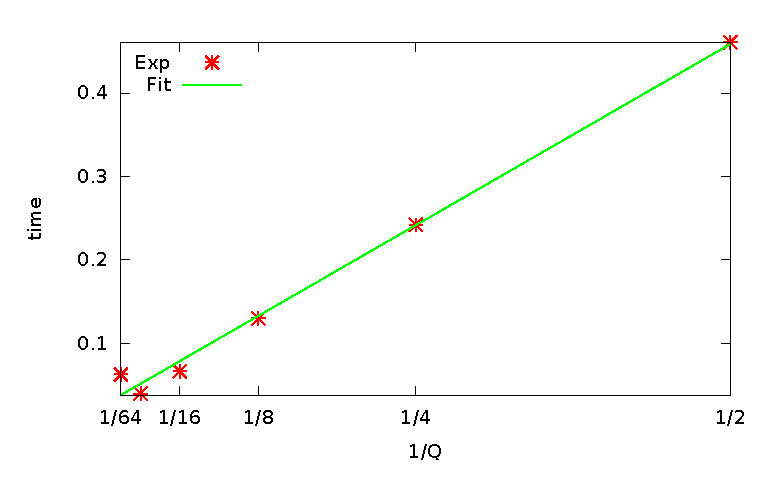
\includegraphics[scale=1.]{t3_exp1.eps}
	\caption{Plot of first set of experiments. The slope is $r M N t_f$, hence $t_f = 8.69$ns.}
	\label{fig1}
\end{figure}

\paragraph{The second set of experiments} we vary $M$ only, and keep $r$, $N$ and $Q$ fixed.  And we can plot a $t_{\textrm{total}} \sim M$ figure.
We also fit this plot by a line. The intercept of this line is $2 r t_s$.  The slope of this line is $r (2 t_w + \frac{N}{Q}t_f)$.
From the intercept and slope, we can get $t_s$ and $t_w$. The setup is that $r=100$, $N=1000$, $Q=32$ and $M=10^3, 2\times10^3, 3\times10^3, 4\times10^3, 5\times10^3$.
The results of the experiments is listed in the Tab \ref{tab3} and is plotted in Fig \ref{fig2} as well. The plot shows very good linearity, and the 
intercept is $3.66\times10^{-3}$, therefore, $t_s = 3.66\times10^{-3}/2/100 = 1.83\times10^{-5}$s. The slope is $3.82\times10^{-5}$, therefore $t_w = (3.82\times10^{-5}/r - \frac{N}{Q}t_f)/2 = 56.5$ns.

\begin{figure}[!htb]
	\centering
	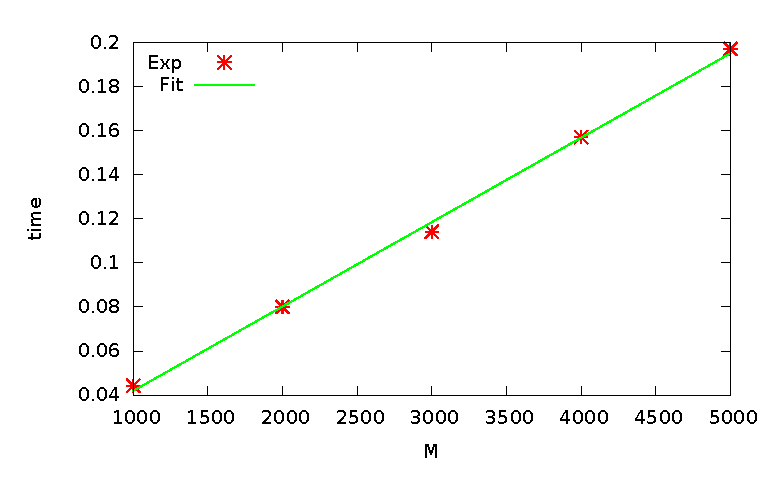
\includegraphics[scale=1.]{t3_exp2.eps}
	\caption{Plot of second set of experiments. The slope is $r (2 t_w + \frac{N}{Q}t_f)$, and intercept is $2 r t_s$ , hence $t_s = 18.3\mu$s, and $t_w=56.5$ns.}
	\label{fig2}
\end{figure}

\begin{table}[h]
	\centering
	\caption{Result of second set of experiments to determine $t_s$ and $t_w$. Varying $M$ and keeping $r, N, Q$ fixed.}
	\label{tab3}
	\begin{tabular}{lllllll}
		\hline
		M                        & $10^3$ & $2\times10^3$ & $3\times10^3$ & $4\times10^3$ & $5\times10^3$ \\ \hline
		$t_{\textrm{total}}$ (s) & $4.42\times 10^{-2}$ & $8.00\times 10^{-2}$ & $1.14\times 10^{-1}$ & $1.57\times 10^{-1}$ & $1.97\times 10^{-1}$ \\ \hline
	\end{tabular}
\end{table}

\subsection{Summary}
So $t_s = 18.3\mu$s, $t_w = 56.5$ns and $t_f = 8.69$ns.
